
\newpage
\subsection*{Задание 2}
	В данном задании использовались:\\
ваттметр типа Д535, блок питания БП типа Б5-9, вольтметр V типа В7-16А, магазин сопротивлений типа МСР.\\
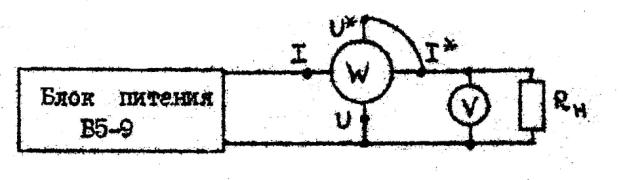
\includegraphics[width=\textwidth]{Part2.png}\\
	При измерении мощности устанавливают на нагрузке напряжение UН=40 В, которое измеряют вольтметром V. После этого измерения сопротивление нагрузки RН и регистрирует показания ваттметра W. Результат измерения заносят в ф.2:\\

	\begin{table} [h!]
 	 \begin{tabular}{|p{6cm}|p{2cm}|p{2cm}|p{2cm}|p{2cm}|}
 	\hline
 	Напряжение $U_{H}$, (В) & 40 & 40 & 40 & 40 \\
 	\hline
 	Сопротиаление $R_{H}$, (Ом) & 500 & 1000 & 1500 & 2000 \\
 	\hline
 	Показания ваттметра $P_{w}$, (Вт) & 3.55 & 1.7 & 1.2 & 0.9 \\
 	\hline
 	Поправка - $\Delta _{P}$, (Вт) & 0.1 & 0.1 & 0.1 & 0.1 \\
 	\hline
 	Мощность нагрузки $P_{H}$, (Bт) & 3.45 & 1.6 & 1.1 & 0.8 \\
 	\hline
 	Погрешность $\delta _{p}$, (\%) & 52.82 & 110.3 & 156.25 & 208.33 \\
 	\hline
 	\end{tabular}
 	\vspace{1cm}
 	Сопротивление нагрузки: $R_{H}$=100 кОм.\\
 	Мощность $P_{Н}$ , потребляемую нагрузкой, вычисляют по формуле $Р_{Н}$ =$P_{w}$ - $\delta$Р.\\
 	Относительную погрешность измерения мощности рассчитывают по формуле:\\
 	$\delta _{p}$ = ($U_{H}$*$I_{H}$*$k_{w}$ $\setminus$ $P_{w}$) * \%
\end{table}
